\documentclass[11pt]{article}
\usepackage[final]{acl}
\usepackage{times}
\usepackage{latexsym}
\usepackage[T1]{fontenc}
\usepackage[utf8]{inputenc}
\usepackage{microtype}
\usepackage{graphicx}
\usepackage{booktabs}
\usepackage{amsmath}
\usepackage{multirow}
\usepackage{tikz}
\usepackage{pgfplots}
\pgfplotsset{compat=1.17}
\usetikzlibrary{arrows.meta,positioning,shapes.geometric,fit,backgrounds}
\usepackage{inconsolata}

\newcommand{\hasans}{\textsc{HasAns}@$k$}

\title{Retrieval Quality Is Not the Bottleneck Until the Prompt Is:\\
       Building GPT-small and a Reranking RAG System for Open-Domain QA}

\author{CSE402 Default Final Project}

\begin{document}
\maketitle

\begin{abstract}
We implement GPT-small, a 63.58M-parameter Transformer decoder with RoPE, grouped-query
attention, RMSNorm and SwiGLU, pretrain it from scratch, and finetune it for summarization,
text classification and retrieval-augmented question answering on Natural Questions.
We then build a retrieval-augmented generation (RAG) system around
\texttt{Llama-3.2-1B-Instruct} and improve it along two axes. First, we show that the
evaluation metric used in this project---containment of the gold answer in the
prediction---systematically rewards verbose outputs, so that accuracy and ROUGE can rank the
same systems in opposite orders; a JSON-constrained chat prompt resolves the tension and
raises accuracy from 0.2451 to 0.2724 and ROUGE-1 from 0.2124 to 0.3332 over the naive
prompt. Second, we rerank a deepened BM25 pool with the generator's own query likelihood,
which lifts the fraction of prompts that actually contain the answer from 0.528 to 0.658.
Deepening that pool further saturates: doubling it to 100 candidates costs 67 extra minutes
for a gain that does not survive a paired test. Two cheaper levers do better. A controlled
experiment that pins the answer-bearing passage to each prompt slot shows a monotone
$16.5$-point recency bias with no middle trough, and simply placing the best evidence last
gains $+1.3$ points at no additional compute; fusing the query-likelihood ranking with the
likelihood of the model's own first-pass answer---two signals correlated at only
$\rho{=}0.14$---adds another $+0.7$. Together they reach 0.3556 accuracy and 0.4191 ROUGE-1,
$+11.1$ and $+20.7$ points over the naive system, at less compute than the deeper pool.
A cheap CPU-only retrieval diagnostic, run before any GPU time
was spent, predicted that reranking would be the effective lever; that prediction held. We
also report three negative results: adaptive context pruning hurts, sentence-level compression
discards the answer when its selector is untrained, and chain-of-thought prompting is the
worst of five prompt variants on this task.
\end{abstract}

\section{Introduction}

Large language models encode world knowledge in their parameters, but that knowledge is fixed
at training time and expensive to update. Retrieval-augmented generation
\citep{lewis2020rag} sidesteps parameter updates by placing evidence in the context window,
and has become standard in deployed systems. Its effectiveness rests on two separable
components: a retriever that must surface evidence containing the answer, and a generator
that must extract the answer from that evidence.

This report covers both halves of the default final project. Part~1 implements GPT-small and
establishes that the implementation is correct by reproducing the reference training curves
supplied with the assignment. Part~2 builds a RAG system and improves it.

Our contributions are:

\begin{enumerate}
\item A GPT-small implementation whose parameter count (63.58M) and pretraining curve match
      the reference log at all six published checkpoints, together with a
      with-versus-without-pretraining comparison on three downstream tasks.
\item A prompt ablation for \texttt{Llama-3.2-1B-Instruct} that isolates a measurement
      artifact: because accuracy is defined as \emph{containment} of the gold string, a
      verbose baseline scores higher accuracy while scoring lower ROUGE. We identify the
      prompt that is best under both metrics simultaneously.
\item A reranking extension that reuses the generator as a zero-shot reranker
      \citep{sachan2022upr}, requiring no new model and no training, and an evaluation
      protocol that reports a retrieval-level metric alongside end accuracy so that
      ``the reranker was bad'' and ``the generator could not use the better context'' remain
      distinguishable.
\item A CPU-only diagnostic that determines, before any GPU time is spent, whether reranking
      can help at all---and a pre-registered decision rule based on it.
\end{enumerate}

\section{Related Work}

\paragraph{Architecture.} GPT-small follows the modern decoder recipe: the Transformer block
of \citet{vaswani2017attention} with rotary position embeddings \citep{su2023roformer},
grouped-query attention \citep{ainslie2023gqa}, RMSNorm \citep{zhang2019rmsnorm} and a SwiGLU
feed-forward network, arranged pre-norm as in Llama.

\paragraph{Retrieval-augmented generation.} \citet{lewis2020rag} introduced RAG with an
encoder--decoder reader; we use a decoder-only reader, as modern systems do. Our retriever is
BM25 through Pyserini \citep{lin2021pyserini} over the DPR Wikipedia split
\citep{karpukhin2020dpr}, evaluated on NQ-open \citep{kwiatkowski2019nq}.

\paragraph{Improving RAG.} Our extension is Unsupervised Passage Reranking
\citep{sachan2022upr}, which scores a passage by the likelihood the language model assigns to
the question given that passage. This is the direct realization of the project guidance to
``select only the most relevant segments by measuring their relevance to the question.''

We deliberately did \emph{not} implement Parallel Context Windows \citep{ratner2023pcw} or
context compression \citep{hou2024compression}, although both were suggested. PCW addresses
models with a limited maximum input length; \texttt{Llama-3.2-1B-Instruct} has a 128k context
window and our prompts are roughly 900 tokens, so the problem PCW solves does not exist in
this configuration. Context compression has the same difficulty in reverse: the retrieval unit
is already a 100-word passage, and compressing it risks deleting the answer span in an
extractive task. Self-RAG \citep{asai2024selfrag} and RAFT \citep{zhang2024raft} both require
training a critic or a domain-adapted reader, which exceeds the compute budget; we borrow only
Self-RAG's inference-time ``should I retrieve?'' idea as a thresholding gate, and report it as
such.

Three recent systems attack the cost of a deep pool from different sides, and each couples its
idea to a trained component we cannot reach on a zero-training budget. EXIT
\citep{hwang2025exit} keeps sentences rather than passages so a deep pool fits a shallow
pool's token budget, but its selector is finetuned on 427K HotpotQA sentence annotations,
which NQ does not have. InfoGain-RAG \citep{wang2025infogain} ranks a document by how much it
raises the likelihood of the \emph{answer} rather than of the question---a quantity defined
over the gold answer, distilled into a reranker whose weights are unreleased. GRAD
\citep{lee2026grad} cancels positional bias with the logits of a debiasing-trained model, having
rejected the training-free alternative of permuting the context as too expensive. We take the
ranking criterion from the second and the positional insight from the third and realize both
without training (\S\ref{sec:combined}); the compression idea we measure but do not adopt
(\S\ref{sec:compression}).

\section{Approach}

\subsection{GPT-small}

The model is a pre-norm Transformer decoder. Writing $x$ for a hidden state, one layer is
\begin{align}
h    &= x + \mathrm{Attn}(\mathrm{RMSNorm}(x)), \\
\mathrm{out} &= h + \mathrm{FFN}(\mathrm{RMSNorm}(h)).
\end{align}

\paragraph{RMSNorm.} $\mathrm{RMSNorm}(x) = \frac{x}{\sqrt{\mathrm{mean}(x^2)+\epsilon}} \odot \gamma$.
The mean of squares is accumulated in fp32 even when the model runs in bfloat16, then cast
back; computing it in bf16 loses precision that the normalization then amplifies.

\paragraph{RoPE.} With $\theta_i = \text{base}^{-2i/d}$ and position $m$, the pair
$(x_1, x_2)$ at frequency $i$ is rotated by $m\theta_i$:
\begin{equation}
[x_1', x_2'] = [x_1\cos - x_2\sin,\; x_1\sin + x_2\cos].
\end{equation}
After rotation, $\langle R_m q, R_n k\rangle$ depends only on $m-n$. We use the
split-halves pairing used by Llama rather than the interleaved pairing of the original paper;
the same permutation is applied to $q$ and $k$, so inner products are unchanged, and the
split-halves form allows numerical comparison against HuggingFace's \texttt{LlamaForCausalLM}.
The $\cos/\sin$ table is computed under \texttt{autocast(enabled=False)} because angle error
at large positions is significant in bf16.

\paragraph{GQA.} 16 query heads share 4 key/value heads, which are repeated to match. This
shrinks the KV cache and the projection parameters. All projections are bias-free: adding
biases yields 63.59M parameters, while omitting them yields exactly the 63.58M reported in the
reference log.

\paragraph{Attention mask.} Causal and padding masks are combined into one additive 4D mask
whose blocked entries are \texttt{finfo(dtype).min} rather than $-\infty$. With left padding,
a padded row can have every key masked; using the dtype minimum makes such a row degenerate to
a uniform distribution instead of producing \texttt{NaN}. With a KV cache the query at index
$i$ has absolute position $\text{seen}+i$, and the mask is shifted accordingly.

\paragraph{Loss.} Logits at position $t$ predict the token at $t+1$, so logits and labels are
shifted by one inside the model; the data collators pass \texttt{labels = input\_ids.clone()}
unshifted. Padding and prompt positions carry $-100$ and are excluded.

\subsection{Task-specific data}

\paragraph{Summarization.} Each example is packed to a fixed 1024 tokens as
\texttt{[pad]\dots[bos] "Context: \dots\textbackslash n Summary:\textbackslash n" summary [eos]},
with $-100$ on everything except the summary and its \texttt{eos}. The length is fixed because
the provided collator builds a tensor directly from a list of lists.

\paragraph{Classification.} The provided preprocessing pads within each 1000-example map
batch, so stored lengths are inconsistent. The collator strips that padding using the
attention mask and re-pads \emph{left} to the batch maximum, because the classification head
reads \texttt{hidden\_states[:, -1, :]} and therefore requires the last position to be a real
token. RoPE is relative, so the position shift introduced by left padding does not change the
result.

\paragraph{RAG finetuning.} Training examples sample up to five gold passages from
\texttt{positive\_ctxs} in the same
\texttt{Title:/Passage:/Question:/Answer:} template the inference path uses, so that a model
with no zero-shot ability sees one consistent format. The passage block is truncated to 768
tokens so that the collator's right-truncation at 992 never removes \texttt{Answer:}.

\subsection{Baseline RAG: prompting \texttt{Llama-3.2-1B-Instruct}}

\begin{figure}[t]
\centering
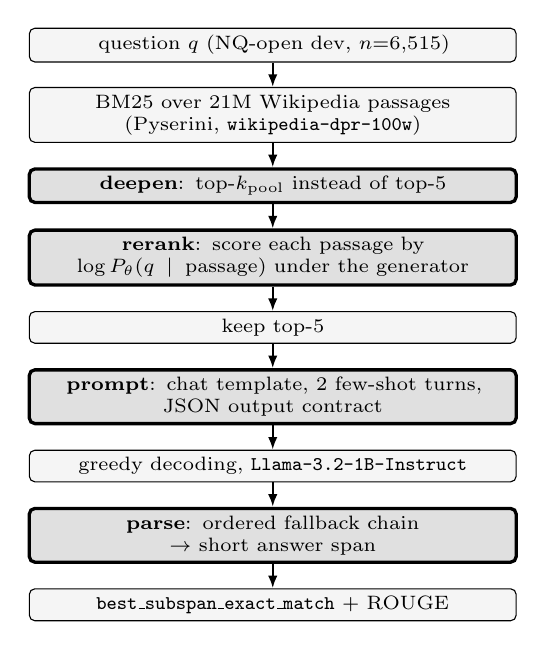
\begin{tikzpicture}[
  node distance=3.1mm,
  box/.style={draw, rounded corners=2pt, align=center, font=\scriptsize,
              inner sep=2.6pt, text width=60mm},
  lit/.style={box, fill=black!4},
  new/.style={box, fill=black!12, very thick},
  arr/.style={-{Latex[length=1.6mm]}, thick}
]
\node[lit] (q) {question $q$ (NQ-open dev, $n{=}6{,}515$)};
\node[lit, below=of q] (bm) {BM25 over 21M Wikipedia passages\\(Pyserini, \texttt{wikipedia-dpr-100w})};
\node[new, below=of bm] (pool) {\textbf{deepen}: top-$k_{\text{pool}}$ instead of top-5};
\node[new, below=of pool] (rr)  {\textbf{rerank}: score each passage by\\$\log P_\theta(q \mid \text{passage})$ under the generator};
\node[lit, below=of rr] (top5) {keep top-5};
\node[new, below=of top5] (pr) {\textbf{prompt}: chat template, 2 few-shot turns,\\JSON output contract};
\node[lit, below=of pr] (gen) {greedy decoding, \texttt{Llama-3.2-1B-Instruct}};
\node[new, below=of gen] (parse) {\textbf{parse}: ordered fallback chain\\$\rightarrow$ short answer span};
\node[lit, below=of parse] (ev) {\texttt{best\_subspan\_exact\_match} + ROUGE};
\draw[arr] (q)--(bm); \draw[arr] (bm)--(pool); \draw[arr] (pool)--(rr);
\draw[arr] (rr)--(top5); \draw[arr] (top5)--(pr); \draw[arr] (pr)--(gen);
\draw[arr] (gen)--(parse); \draw[arr] (parse)--(ev);
\end{tikzpicture}
\caption{The proposed system. Shaded boxes are the components we add; the rest is the
provided pipeline. Reranking adds no new model---the generator scores its own retrieval.}
\label{fig:system}
\end{figure}

\paragraph{The metric determines the design.} Accuracy in this project is
\texttt{best\_subspan\_exact\_match}: a prediction is correct when a normalized gold answer is
a \emph{substring} of the normalized prediction. Three consequences follow directly.
(i) Long predictions are rewarded, because a longer string is more likely to contain the gold
span. (ii) ROUGE, being an F-measure against a one-to-five word gold answer, punishes exactly
the same verbosity. (iii) An empty prediction is counted wrong unconditionally. Therefore
abstention is never rational under this metric, and we instruct the model to guess rather
than decline; this is the opposite of normal RAG practice and we flag it as an artifact of the
evaluation rather than a recommendation.

\paragraph{Prompt variants.} We evaluate five variants that differ in exactly one factor at a
time. \textsc{V0} keeps the provided plain-completion prompt and changes only the decoding
settings, isolating the effect of prompting from the effect of decoding. \textsc{V1} adds the
Llama chat template and a terse-answer instruction. \textsc{V2} adds two few-shot user/assistant
turns. \textsc{V3} additionally constrains the output to \texttt{\{"answer": "\dots"\}}.
\textsc{V4} replaces the format contract with a length-bounded two-line chain of thought
\citep{wei2022cot}. All variants decode greedily.

\paragraph{Parsing.} Instruction-tuned models wrap answers in prose. Our parser applies an
ordered chain: strip special-token residue; truncate at any hallucinated next turn
(\texttt{\textbackslash nQuestion:}, \texttt{\textbackslash nTitle:}, \dots); remove greetings,
answer labels and markdown; drop trailing justification clauses; cap at twelve words. JSON
outputs get a dedicated chain with regex repair for unterminated braces and single quotes. The
chain has one invariant: \emph{a non-empty generation never parses to an empty prediction},
because an empty prediction is a guaranteed miss while a malformed string may still contain
the answer. The chain is unit-tested on 29 cases without a GPU.

\paragraph{Two defects in the provided evaluation path.} The chat template already emits
\texttt{<|begin\_of\_text|>}, so tokenizing its output with \texttt{add\_special\_tokens=True}
produces a duplicate BOS; we disable it. Separately, \texttt{eval\_for\_rag} passes the GPT-2
tokenizer's \texttt{eos\_token\_id} (50256) as Llama's \texttt{pad\_token\_id}, and 50256 is an
ordinary text token in Llama's vocabulary, so \texttt{skip\_special\_tokens} does not remove
it and it is appended after short answers. We override both inside our subclass rather than
editing the provided cell, so the original naive numbers remain reproducible.

\subsection{Extension: query-likelihood reranking}

BM25 retrieves top-$k_{\text{pool}}$ rather than top-5. Each candidate is scored by the mean
log-likelihood the generator assigns to the question given the passage,
\begin{equation}
s(p) = \frac{1}{|q|}\sum_{t} \log P_\theta\!\left(q_t \mid q_{<t}, \text{prompt}(p)\right),
\end{equation}
using a plain completion prompt (``\texttt{Passage: \dots{} Please write a question based on
this passage. Question:}''). The top-5 by $s$ enter the generation prompt. Dividing by $|q|$
does not change the ranking within a question---the scored tokens are identical---but puts
questions on a common scale, which the assembly variant below depends on.

The cost is forward passes only, no decoding, and no second model. To keep it affordable we
slice the logits to the question positions \emph{before} the \texttt{float()} upcast; with a
128k vocabulary the full logit tensor would otherwise dominate memory.

We also evaluate an adaptive assembly variant that uses the same scores to choose how many
passages to include (cumulative softmax mass $\tau$), in which order, and whether to drop the
context entirely. Its softmax temperature is set from the score spread so that one threshold
works for both BM25 scores ($\approx +20$) and mean log-likelihoods ($\approx -2.5$).

\subsection{Prompt position and answer likelihood}
\label{sec:combined}

Two further mechanisms act on the same reranked pool and are free of any training.

\paragraph{Slot order.} The reranked top-5 is permuted before it enters the prompt. This adds
no forward passes and changes no retrieval: the set of passages, and therefore \textsc{HasAns},
is held exactly fixed. We compare rank order, its reverse, and two edge arrangements that put
the best evidence at the first and last slot. The choice is made from a controlled measurement
of where the reader actually reads (\S\ref{sec:position}), not from the literature.

\paragraph{Answer likelihood without gold.} InfoGain-RAG's criterion needs the gold answer, so
it cannot run at inference. We substitute the first-pass prediction $\hat{y}$ of the best
position-ordered system and score each candidate by
\begin{equation}
s_a(p) = \frac{1}{|\hat{y}|}\sum_{t}\log P_\theta\!\left(\hat{y}_t \mid \hat{y}_{<t},
\text{prompt}(p, q)\right).
\end{equation}
A first pass that is right 35\% of the time makes $s_a$ noisy on its own, so the UPR and $s_a$
rankings are combined by reciprocal rank fusion, $\sum_r 1/(60 + \text{rank}_r(p))$, which
degrades gracefully when one input is noisy. Score vectors are cached per passage, so
configurations sharing a pool pay for scoring once. The original formulation's no-document
baseline term is constant within a query and cannot change the ranking; we compute it only to
report the sign.

\subsection{A diagnostic that runs before any GPU time}

\begin{figure}[t]
\centering
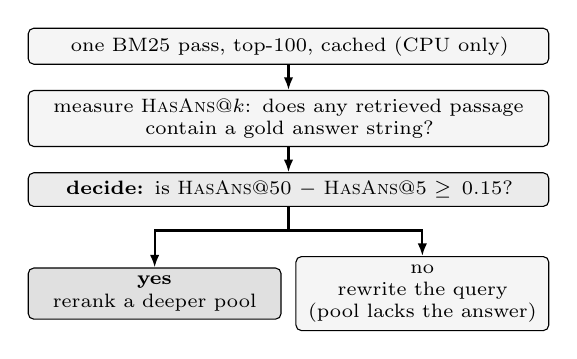
\begin{tikzpicture}[
  node distance=3.2mm,
  b/.style={draw, rounded corners=2pt, align=center, font=\scriptsize, inner sep=3pt,
            text width=64mm},
  s/.style={draw, rounded corners=2pt, align=center, font=\scriptsize, inner sep=3pt,
            text width=30mm},
  d/.style={draw, rounded corners=2pt, align=center, font=\scriptsize, inner sep=3pt,
            text width=64mm, fill=black!8},
  arr/.style={-{Latex[length=1.6mm]}, thick}
]
\node[b, fill=black!4] (p) {one BM25 pass, top-100, cached (CPU only)};
\node[b, below=of p, fill=black!4] (m)
  {measure \hasans{}: does any retrieved passage\\contain a gold answer string?};
\node[d, below=of m] (c)
  {\textbf{decide:} is \textsc{HasAns}@50 $-$ \textsc{HasAns}@5 $\ge 0.15$?};
\node[s, fill=black!12] (y) at ([xshift=-17mm, yshift=-11mm]c.south)
  {\textbf{yes}\\rerank a deeper pool};
\node[s, fill=black!4] (n) at ([xshift=17mm, yshift=-11mm]c.south)
  {no\\rewrite the query\\(pool lacks the answer)};
\draw[arr] (p)--(m);
\draw[arr] (m)--(c);
\draw[arr] (c.south) -- ++(0,-3mm) -| (y.north);
\draw[arr] (c.south) -- ++(0,-3mm) -| (n.north);
\end{tikzpicture}
\caption{Pre-registered decision rule. The measured gap was $0.2728$, selecting the
reranking branch before any GPU time was committed.}
\label{fig:diag}
\end{figure}

Before running the extension we measured, on CPU alone, how much headroom a reranker could
possibly have. We define \hasans{} as the fraction of questions for which at least one of the
top-$k$ retrieved passages contains a normalized gold answer string. This is an upper bound on
extractive accuracy at that $k$, and unlike gold-passage recall it is not biased by the fact
that DPR's \texttt{positive\_ctxs} were themselves selected from BM25 output. We pre-registered
the rule in Figure~\ref{fig:diag}: reranking is worth trying only if the pool contains
substantially more answers than the top-5 does.

\section{Experiments}

GPT-small uses 4 layers, hidden size 512, intermediate size 2048, 16 query heads, 4 key/value
heads, head dimension 32, context length 1024 and $\theta_{\text{rope}}=20000$, trained in pure
bfloat16. Pretraining runs 2 epochs on \texttt{cosmopedia-v2}; summarization 3 epochs on
CNN/DailyMail; classification 5 epochs on 20 Newsgroups; RAG 3 epochs on NQ. All RAG evaluation
uses the full NQ-open dev set ($n=6{,}515$) and greedy decoding, so a single run per
configuration is reproducible and seed averaging is unnecessary.

\paragraph{Environment deviations.} The assignment specifies PyTorch 2.6.0. Our GPU is an RTX
5080 (Blackwell, \texttt{sm\_120}); the 2.6.0 CUDA 12.4 wheels are compiled for
\texttt{sm\_50}--\texttt{sm\_90} only and every matrix multiplication fails with
\emph{no kernel image is available for execution on the device}. We therefore used PyTorch
2.7.1 with CUDA 12.8, which is the earliest release supporting this architecture. We kept
\texttt{transformers} pinned at 4.52.4: from 4.54 onwards \texttt{lm\_head} is automatically
tied to the input embedding, which changes the model to 39.04M parameters and breaks
\texttt{save\_pretrained}.

With 16\,GB of VRAM the notebook's micro-batch of 16 does not fit (measured peak 10.95\,GiB at
batch 8; batch 12 exhausts memory). We used micro-batch 8 and \emph{scaled gradient
accumulation and both logging intervals by the same factor}. Because the training loop counts
\texttt{global\_steps} in micro-batches, this keeps the effective batch (32), the learning-rate
schedule and the token position of every evaluation identical to the reference configuration;
throughout this report we quote reference-equivalent steps.

\section{Results}

\subsection{GPT-small pretraining}

The implementation reproduces the reference log at every published checkpoint
(Table~\ref{tab:pretrain}); all six points agree to within bf16 rounding. This is
simultaneously evidence that the architecture is correct and that the batch rescaling above
preserved the training mathematics. Figure~\ref{fig:curves} shows the full run.

\begin{table}[t]
\centering\small
\begin{tabular}{@{}rccc@{}}
\toprule
step & reference & ours & $\Delta$ \\
\midrule
2{,}500  & 4.47 / 87.50 / .309 & 4.50 / 91.50 / .306 & \textminus.003 \\
5{,}000  & 3.73 / 42.25 / .366 & 3.75 / 43.00 / .364 & \textminus.002 \\
7{,}500  & 3.48 / 33.00 / .389 & 3.50 / 33.75 / .387 & \textminus.002 \\
10{,}000 & 3.36 / 29.00 / .404 & 3.38 / 29.38 / .402 & \textminus.002 \\
12{,}500 & 3.28 / 26.75 / .412 & 3.28 / 26.88 / .411 & \textminus.001 \\
15{,}000 & 3.22 / 25.25 / .419 & 3.22 / 25.38 / .418 & \textminus.001 \\
\midrule
93{,}843 & --- & 3.00 / 20.38 / .449 & --- \\
\bottomrule
\end{tabular}
\caption{Pretraining: loss / perplexity / token accuracy against the reference log. $\Delta$
is on token accuracy. Model size is 63.58M parameters, matching the reference exactly.}
\label{tab:pretrain}
\end{table}

\begin{figure}[t]
\centering
\begin{tikzpicture}
\begin{axis}[
  width=0.94\columnwidth, height=4.1cm,
  xlabel={reference-equivalent step}, ylabel={loss},
  xmin=0, xmax=95000, ymin=2.8, ymax=7,
  tick label style={font=\scriptsize}, label style={font=\scriptsize},
  legend style={font=\scriptsize, at={(0.97,0.97)}, anchor=north east, draw=none,
                fill=white, fill opacity=0.8, text opacity=1},
  grid=major, grid style={black!10},
]
\addplot[thick, black!55] table {data_pre_train.dat};
\addlegendentry{train (running mean)}
\addplot[thick, black, mark=*, mark size=0.7] table[x index=0, y index=1] {data_pre_eval.dat};
\addlegendentry{eval}
\end{axis}
\end{tikzpicture}
\begin{tikzpicture}
\begin{axis}[
  width=0.94\columnwidth, height=3.5cm,
  xlabel={reference-equivalent step}, ylabel={token accuracy},
  xmin=0, xmax=95000, ymin=0.28, ymax=0.47,
  tick label style={font=\scriptsize}, label style={font=\scriptsize},
  grid=major, grid style={black!10},
]
\addplot[thick, black, mark=*, mark size=0.7] table[x index=0, y index=3] {data_pre_eval.dat};
\end{axis}
\end{tikzpicture}
\caption{Pretraining progress over two epochs. Evaluation loss appears to freeze at 3.00 late
in training; this is bf16 quantization of the logged scalar---token accuracy, computed in
fp32, still moves in the sixth decimal, and the cosine schedule ends at a learning rate of
$3.5\times10^{-13}$.}
\label{fig:curves}
\end{figure}

\subsection{Downstream tasks, with and without pretraining}

Table~\ref{tab:pretrainablation} compares finetuning from the pretrained checkpoint against
finetuning an identically configured but randomly initialized model for the same number of
steps. The effect is large on all three tasks and dramatic on RAG, where the random model
answers essentially nothing. Summarization degrades from ROUGE-1 0.1790 to 0.0639 and its
evaluation loss rises from 3.938 to 6.536; ROUGE-2 collapses by a factor of thirteen
($0.0367 \rightarrow 0.0028$), so the random-init model produces almost no correct bigrams
at all and its apparent unigram overlap is largely incidental.

\begin{table}[t]
\centering\small
\begin{tabular}{@{}llccc@{}}
\toprule
task & metric & pretrained & random & $\Delta$ \\
\midrule
20NG    & acc.    & \textbf{0.5917} & 0.3093 & $+0.2824$ \\
CNN/DM  & ROUGE-1 & \textbf{0.1790} & 0.0639 & $+0.1151$ \\
CNN/DM  & ROUGE-2 & \textbf{0.0367} & 0.0028 & $+0.0339$ \\
NQ RAG  & acc.    & \textbf{0.0480} & 0.0054 & $+0.0427$ \\
NQ RAG  & ROUGE-1 & \textbf{0.0877} & 0.0217 & $+0.0660$ \\
\bottomrule
\end{tabular}
\caption{Effect of pretraining on downstream finetuning. Each control finetunes an
identically configured but randomly initialised checkpoint for the same number of steps.}
\label{tab:pretrainablation}
\end{table}

Summarization reaches ROUGE-1 0.1790 / ROUGE-2 0.0367 / ROUGE-L 0.1405. The generations are
fluent but repetitive---one sample repeats \emph{``The Israeli Court is also a step forward to
the Constitution''} verbatim twice and then once more with the subject swapped
(\emph{``The U.S. is a step forward to the Constitution''})---which the very low ROUGE-2
quantifies. RAG finetuning peaks
at accuracy 0.0480, against a reference value of 0.0328 at the one published checkpoint (we
measure 0.0356 there). Its predictions show that the 63.58M model learns the \emph{format}
perfectly but not the content: for \emph{``where do the great lakes meet the ocean''} it
answers \emph{``New York State Canal''}---a plausible entity of the right type and length, and
wrong. This is precisely the gap that motivates moving to an instruction-tuned model.

\subsection{Prompting and extensions}

\begin{table*}[t]
\centering\small
\begin{tabular}{@{}llccccrr@{}}
\toprule
& system & acc. & ROUGE-1 & ROUGE-2 & ROUGE-L & \textsc{HasAns} & words \\
\midrule
& naive RAG (provided cell) & 0.2451 & 0.2124 & 0.1129 & 0.2109 & --- & --- \\
\midrule
\multirow{5}{*}{\rotatebox{90}{\S4.2.1}}
& \textsc{V0} plain prompt, controlled decoding & 0.3176 & 0.2524 & 0.1459 & 0.2508 & 0.528 & 7.34 \\
& \textsc{V1} chat template, zero-shot          & 0.2021 & 0.2577 & 0.1444 & 0.2567 & 0.528 & 1.80 \\
& \textsc{V2} \quad + 2 few-shot turns          & 0.2118 & 0.2890 & 0.1399 & 0.2881 & 0.528 & 1.60 \\
& \textsc{V3} \quad + JSON contract \textbf{(baseline RAG)} & 0.2724 & 0.3332 & 0.1777 & 0.3321 & 0.528 & 1.89 \\
& \textsc{V4} \quad + two-line CoT              & 0.1948 & 0.2509 & 0.1289 & 0.2506 & 0.528 & 1.79 \\
\midrule
\multirow{5}{*}{\rotatebox{90}{\S4.3}}
& \textsc{V2} + rerank ($k_{\text{pool}}{=}20$)      & 0.2451 & 0.3272 & 0.1625 & 0.3265 & 0.625 & 1.63 \\
& \textsc{V2} + adaptive assembly                    & 0.1975 & 0.2654 & 0.1374 & 0.2648 & 0.442 & 1.63 \\
& \textsc{V2} + rerank + assembly                    & 0.2405 & 0.3205 & 0.1658 & 0.3194 & 0.554 & 1.63 \\
& \textsc{V3} + rerank ($k_{\text{pool}}{=}20$)      & 0.3213 & 0.3828 & 0.2104 & 0.3818 & 0.625 & 1.93 \\
& \textsc{V3} + rerank ($k_{\text{pool}}{=}50$) \textbf{(proposed)} & 0.3361 & 0.3978 & 0.2221 & 0.3969 & 0.658 & 1.93 \\
& \textsc{V3} + rerank ($k_{\text{pool}}{=}100$) & 0.3431 & 0.4052 & 0.2248 & 0.4042 & \textbf{0.664} & 1.94 \\
\midrule
\multirow{4}{*}{\rotatebox{90}{\S\ref{sec:combined}}}
& \quad + best evidence last                         & 0.3489 & 0.4142 & 0.2323 & 0.4128 & 0.658 & 1.93 \\
& \quad + answer-likelihood fusion                   & 0.3434 & 0.4090 & 0.2293 & 0.4079 & 0.607 & 1.92 \\
& \quad + fusion, $k_{\text{pool}}{=}20$             & 0.3392 & 0.4024 & 0.2239 & 0.4012 & 0.587 & 1.93 \\
& \quad + fusion + last \textbf{(proposed)} & \textbf{0.3556} & \textbf{0.4191} & \textbf{0.2378} & \textbf{0.4180} & 0.607 & 1.95 \\
\midrule
& \emph{oracle answer likelihood (not a system)} & \emph{0.4698} & \emph{0.5420} & \emph{0.2997} & \emph{0.5406} & \emph{0.766} & 1.91 \\
\bottomrule
\end{tabular}
\caption{Full NQ-open dev set ($n=6{,}515$), greedy decoding. \textsc{HasAns} is the fraction
of prompts whose passages contain a gold answer string---a retrieval-side metric that is
independent of the generator. ``words'' is the mean prediction length, which explains most of
the accuracy/ROUGE disagreement.}
\label{tab:main}
\end{table*}

Table~\ref{tab:main} gives the full results. The best configuration improves on the naive RAG
system by $+11.1$ accuracy points and $+20.7$ ROUGE-1 points, and on the baseline RAG system
(\textsc{V3}) by $+8.3$ and $+8.6$ points. The proposed operating point is neither of the
deep-pool rows but the fused, position-ordered system at $k_{\text{pool}}{=}50$, for the
reasons given in \S\ref{sec:saturation}.

\section{Analysis}

\paragraph{Accuracy and ROUGE disagree, and length explains it.} \textsc{V0}---the provided
prompt with only decoding and parsing changed---attains the second-highest accuracy in the
table (0.3176) while sitting near the bottom on ROUGE-1 (0.2524). Its mean prediction is 7.34
words, roughly four times longer than every chat-template variant. Under a containment
metric, length is close to free accuracy; under an F-measure against a one-to-five word gold
answer, it is expensive. A reader who looked only at accuracy would conclude that the chat
template hurts. A reader who looked only at ROUGE would conclude the opposite. The
\emph{proposed} system resolves the tension: it is best on both metrics at once, with a mean
length of 1.93 words. We consider this the most important methodological point in the report,
and the reason we report mean prediction length in every row.

\paragraph{Retrieval improved substantially; the generator used only part of it.} Reranking
lifts \textsc{HasAns} from 0.528 to 0.625 at $k_{\text{pool}}{=}20$ and 0.658 at 50---a
retrieval-side gain of up to $13.0$ points that involves no generation at all. End accuracy
moves far less. Reporting both numbers is what makes this interpretable: the reranker is not
failing, the 1B generator is simply unable to convert all of the additional evidence into
correct answers. Had we reported accuracy alone, a modest end gain would have been
indistinguishable from a broken reranker.

\paragraph{Retrieval and prompting interact.} The same reranker, applied to two different
prompts, transfers differently: on \textsc{V2} it buys $+3.3$ accuracy points
($0.2118 \rightarrow 0.2451$), on \textsc{V3} it buys $+4.9$ ($0.2724 \rightarrow 0.3213$).
The retrieval improvement is identical by construction---\textsc{HasAns} is 0.625 in both
cases---so the difference is entirely in how well the prompt lets the model exploit the
evidence. Retrieval quality and prompt quality are not additive, and tuning them separately
understates the combination.

\paragraph{The diagnostic paid for itself.} The measured gap
$\textsc{HasAns}@50 - \textsc{HasAns}@5 = 0.2728$ cleared the pre-registered threshold of
$0.15$ by a wide margin, and 18.9\% of questions have their first answer-bearing passage at
rank 6--20, outside the default top-5. All of this was known before any GPU time was spent on
the extension, and it correctly selected reranking over query rewriting.

\paragraph{Pool depth saturates.}
\label{sec:saturation}
Against the oracle at each depth, reranking recovers a steadily \emph{smaller} share of the
available headroom even as the headroom itself grows:

\begin{center}\small
\begin{tabular}{@{}rcccc@{}}
\toprule
$k_{\text{pool}}$ & \textsc{HasAns} & oracle & recovered & acc. \\
\midrule
5 (none) & 0.528 & --- & --- & 0.2724 \\
20  & 0.625 & 0.717 & 51.1\% & 0.3213 \\
50  & 0.658 & 0.801 & 47.5\% & 0.3361 \\
100 & 0.664 & 0.848 & 42.6\% & 0.3431 \\
\bottomrule
\end{tabular}
\end{center}

Going from 20 to 50 buys $+3.3$ points of \textsc{HasAns}; going from 50 to 100 buys only
$+0.6$. A 1B model scoring by query likelihood becomes a weaker discriminator as the candidate
set grows, so the extra true positives it must promote from ranks 51--100 mostly stay buried.
End accuracy still improves slightly ($+0.7$ points), but scoring cost is linear in
$k_{\text{pool}}$: the $k_{\text{pool}}{=}100$ run took 108 minutes against roughly 20 for
$k_{\text{pool}}{=}20$. The $+0.7$ point gain is in fact not significant on the paired test
($z{=}1.73$, $p{=}0.083$), so doubling the pool buys 67 minutes of compute and no measurable
accuracy. Depth is the wrong lever; the next two paragraphs identify two that work.

\paragraph{The reader has a strong recency bias, and it is not lost-in-the-middle.}
\label{sec:position}
We pinned the answer-bearing passage to one prompt slot and filled the other four with the
highest-ranked passages that do \emph{not} contain the answer, so that position is the only
variable. Over the 5,158 questions where this is possible, accuracy rises monotonically with
slot index: $0.3009$, $0.3275$, $0.3532$, $0.4230$, $0.4663$ for slots one through five. The
last slot beats the first by $16.5$ points ($z{=}24.7$). There is no middle trough. An
uncontrolled reading of the same data suggests one---the first slot looks strong---but that is
a difficulty confound: a question whose answer sits at BM25 rank 1 is an easy question. Once
difficulty is held fixed the first slot is the \emph{worst} place to put the evidence.

This is not a refutation of \citet{liu2024lost}, whose U-shaped curve is what the
uncontrolled reading resembles, but a different regime: they inject a gold document among
10--30 in much larger readers, while our prompt holds five passages and the reader is a 1B
model. With five slots there may be too little middle for a trough to form. The relevant
lesson is methodological---we matched an observational shape to a claim established by
controlled injection, and only the controlled version of our own data settled it.

This predicts the intervention and its failure mode. Moving the best passage to the last slot
gains $+1.27$ points ($z{=}2.98$, $p{=}0.003$) at zero additional compute, while the
edge arrangement that puts the best passage first gains nothing ($+0.08$, $p{=}0.84$)---there
is recency but no primacy to exploit.

The experiment supports ``best evidence last'' and nothing more: it contained exactly one
relevant passage, so it says nothing about arranging the other four. Three arrangements that
place the top passage last span $0.3472$--$0.3556$ and are not reliably separable (the two
extremes differ by $p{=}0.05$ with fusion and $p{=}0.62$ without, an inconsistency that points
to noise). We report the best-measured arrangement but treat only the last-slot placement as
supported.

\paragraph{Two comparable rankers that disagree beat either alone.} Ranking the same pool by
the likelihood of the \emph{gold} answer reaches $0.4698$, $13.4$ points above UPR, and the
two score vectors correlate at only $\rho{=}0.14$ (Spearman, per query). The signal UPR misses
is therefore real and large. Replacing gold with a first-pass prediction recovers part of it:
the substituted ranker alone scores $0.3507$, statistically indistinguishable from UPR's
$0.3489$ ($p{=}0.52$), and fusing the two reaches $0.3556$. The two contributions are additive
and each is significant against the other's ablation---fusion adds $+0.68$ points over
ordering alone ($p{=}0.022$) and ordering adds $+1.23$ over fusion alone ($p{=}0.0006$).

Splitting accuracy by whether the gold string was in the prompt shows what is being traded:

\begin{center}\small
\begin{tabular}{@{}lcccc@{}}
\toprule
ranker & \textsc{HasAns} & acc.\ $\mid$ in & acc.\ $\mid$ out & overall \\
\midrule
UPR          & \textbf{0.658} & 0.520 & 0.019 & 0.3487 \\
answer-lik.  & 0.569 & \textbf{0.606} & 0.014 & 0.3506 \\
fusion       & 0.607 & 0.578 & 0.011 & \textbf{0.3555} \\
\bottomrule
\end{tabular}
\end{center}

UPR puts the answer string in $8.9$ points more prompts but the reader extracts it $8.6$
points less often. ``Contains the answer string'' and ``lets the reader produce the answer''
are different properties, which is InfoGain-RAG's premise, measured here directly. Fusion
takes the middle of both columns and wins the product.

\paragraph{A better ranker substitutes for a deeper pool.} With fusion at
$k_{\text{pool}}{=}20$, accuracy is $0.3392$---statistically tied with UPR at
$k_{\text{pool}}{=}100$ ($p{=}0.45$) at 35 minutes against 108. The proposed system keeps
$k_{\text{pool}}{=}50$ and reaches $0.3556$ in 77 minutes, beating $k_{\text{pool}}{=}100$ by
$1.25$ points while costing 31 minutes less. Depth still helps once the ranker is better
(fusion at 50 beats fusion at 20 by $1.64$ points, $z{=}4.46$), but its returns arrive much
later. We therefore replace $k_{\text{pool}}{=}50$ with the fused, position-ordered system as
the proposed operating point.

The remaining $11.4$ points to the oracle are not reachable this way: a first pass that is
right 35\% of the time supplies a wrong target two thirds of the time, and passages supporting
that wrong target are promoted---visible as \textsc{HasAns} falling from $0.658$ to $0.607$.
Closing it requires the trained reranker that InfoGain-RAG distils, which is not released.

\paragraph{Negative result: sentence compression loses the answer.}
\label{sec:compression}
We implemented EXIT's selection---score each sentence with its own passage as context, one
forward pass per sentence, reassemble in original order---with the untrained generator in
place of the finetuned classifier and a per-question token budget in place of the absolute
threshold, since an uncalibrated scorer at $\tau{=}0.5$ compresses almost nothing. Compression
worked: 20 passages (${\approx}2{,}900$ tokens) reduced to the 731-token budget of the top-5
context they replace, 24 of 110 sentences kept. But \textsc{HasAns} fell from $0.725$ to
$0.55$ on a 40-question probe: the untrained selector discards answer-bearing sentences, the
recall failure the original paper itself reports for frozen scorers. At 110 forward passes per
question (104 minutes) against a signal moving the wrong way we stopped, reaching one level
down the same conclusion \S2 reaches for passage-level compression.

\paragraph{Negative result: adaptive assembly hurts.} Pruning the context to a mean of 2.88
passages drops \textsc{HasAns} to 0.442 and accuracy to 0.1975, below its own baseline, and
the combined variant (0.2405) is worse than reranking alone (0.2451). With prompts of roughly
900 tokens there is no length pressure to relieve, so discarding passages only loses evidence.
The abstain gate was left disabled for the same reason: under a containment metric, declining
to answer is a guaranteed miss.

\paragraph{Negative result: chain-of-thought is the worst variant.} \textsc{V4} is last on
every metric. NQ with BM25 passages is single-hop extraction---there is little to reason
about---and a 1B model's reasoning chain adds failure modes rather than removing them. It also
costs six times the decoding budget. We report this as a finding rather than omitting it.

\paragraph{Parsing robustness.} Across all five prompt variants at $n=6{,}515$, the primary
parse path succeeded for 98.7--99.9\% of generations, and no configuration produced a single
empty prediction. The JSON variant required regex repair 84 times (1.3\%), which is the
measured cost of imposing a format contract on a 1B model; the chain-of-thought variant hit
its token budget without emitting an \texttt{Answer:} line 14 times (0.2\%), indicating the
96-token budget was adequate.

\section{Conclusion}

We built GPT-small and reproduced the reference pretraining curve at every published
checkpoint, then showed that pretraining is worth $+28$ accuracy points on 20 Newsgroups, a factor of
nine on NQ RAG and a factor of thirteen in summarization ROUGE-2. On the RAG side, the largest single lesson is that the evaluation
metric shapes the conclusion: containment accuracy rewards verbosity, so prompt changes that
plainly improve answer quality can appear to hurt. Reporting mean prediction length alongside
both metrics makes this visible. Our proposed system---a JSON-constrained chat prompt over a
BM25 pool ranked by fusing the generator's query likelihood with the likelihood of its own
first-pass answer, with the best evidence placed last---reaches 0.3556 accuracy and 0.4191
ROUGE-1 against 0.2451 and 0.2124 for the naive system, while adding no new model and no
training. The second lesson is that deepening the candidate pool was the wrong lever: doubling
it to 100 costs 67 extra minutes for a gain that does not survive a paired test, whereas
reordering the prompt costs nothing and reranking by answer likelihood costs less than the
deeper pool. Both followed from measurements---a 16.5-point controlled position effect and a
$\rho{=}0.14$ correlation between the two ranking signals---rather than from the papers that
suggested them, whose trained components we could not use. Finally, a CPU-only retrieval
diagnostic correctly predicted that reranking would be the effective lever, at a cost of
minutes rather than GPU-hours; we would run it first again.

\bibliography{custom}

\appendix

\section{Implementation notes}
\label{sec:appendix}

\paragraph{Reproducing on a memory-limited machine.} The provided
\texttt{donwload\_dataset\_nq\_open\_dpr} loads the 7.37\,GB DPR NQ training file with
\texttt{pandas.read\_json} and then copies it to Arrow with \texttt{Dataset.from\_pandas};
the copy needs well over 20\,GB of RAM and is OOM-killed on a 24\,GB machine. We added
\texttt{prepare\_nq\_train.py}, which streams the JSON array with
\texttt{JSONDecoder.raw\_decode}, keeps only the fields \texttt{RAGDataset} reads, and writes
the dataset to the path the provided code expects, so that the provided file is not modified
and simply reports ``Dataset already exists''. The result has the 58,880 rows the assignment
specifies and occupies 314\,MB.

\paragraph{A packaging defect in \texttt{pyserini}.} \texttt{pyserini} 0.44.0 constructs an
\texttt{openai.OpenAI} client at import time in \texttt{pyserini/encode/\_openai.py}, which is
reached transitively by \texttt{from pyserini.search.lucene import LuceneSearcher}. Without an
\texttt{OPENAI\_API\_KEY} in the environment, every RAG case aborts with an OpenAI credentials
error even though only BM25 is used. Setting any placeholder value fixes it; the encoder is
never called.

\paragraph{Generation settings.} All variants use greedy decoding with
\texttt{temperature} and \texttt{top\_p} explicitly cleared, and stop on both
\texttt{<|end\_of\_text|>} and \texttt{<|eot\_id|>}. \texttt{max\_new\_tokens} is 16 for
\textsc{V0}--\textsc{V2}, 32 for \textsc{V3} (JSON scaffolding consumes roughly eight tokens)
and 96 for \textsc{V4}. The chat template is rendered with a fixed \texttt{date\_string},
because Llama's template otherwise interpolates the current date into the system block and
silently changes the prompt between runs.

\paragraph{Reproducibility.} Every number in this report comes from a single greedy run on the
full dev set; there is no sampling and therefore no seed averaging. The reference naive-RAG
numbers quoted from the assignment were measured with Llama's default sampling configuration
and are not directly comparable for that reason.

\end{document}
